\documentclass[10pt]{scrarticle}
\usepackage[utf8]{inputenc}
\usepackage[parfill]{parskip}
\usepackage[T1]{fontenc}
\usepackage[ngerman]{babel}
\usepackage{multirow}
\usepackage{placeins}
\usepackage[official]{eurosym}
\usepackage{listings}
\usepackage{geometry}
\geometry{a4paper, margin=2.5cm}
\usepackage{graphicx}
\graphicspath{ {./images/} }
\usepackage{tabularx}
\usepackage{makecell}

\renewcommand{\familydefault}{\sfdefault}

\title{Entwicklung eines webbasierten ePortfolios}
\subtitle{im Rahmen einer Umschulung zum Fachinformatiker - Anwendungsentwicklung}
\author{Moritz Mandler \& Didier Zielke}
\date{\today}

\begin{document}

\maketitle

%Hier müssen noch weitere Daten rein (siehe Merkblat der HK Hamburg):
%Berufsbezeichnung, Ausbilder, Ausbildungsbetrieb (mit Adresse)

\vspace{\fill}
\textbf{Ausbildungsbetrieb:}\newline
BFW Berufsförderungswerk Hamburg \newline
Marie-Bautz-Weg ??? \newline
22159 Hamburg

\textbf{Ausbilder:}\newline
Petra Treubel \newline
Dr. Olaf Kubillus

\newpage

\tableofcontents

\newpage

\section{Einführung}

Die IT-Solution \& Design GmbH ist eine Lernfirma innerhalb des Berufsförderungswerks Hamburg GmbH (BFW). Als norddeutsches Zentrum für berufliche Rehabilitation und Integration ist das BFW Hamburg kompetenter Partner für Unternehmen, Träger der beruflichen Rehabilitation und Versicherungen und vor allem für Menschen, die aus gesundheitlichen Gründen ihre bisherige Tätigkeit nicht mehr ausüben können.  
Es soll eine einfache Plattform zur Veröffentlichung einer 'Mappe' der eigenen Arbeitsergebnisse geboten werden. Benutzer müssen sich authentifizieren und können dann die eigene Mappe bearbeiten. Innerhalb dieser Mappe, die hier nur eine Webseite darstellt, können beliebige Download-Dateien, Texte und Bilder eingefügt werden. So soll den Benutzern auch die Möglichkeit gegeben werden Lebensläufe, Arbeitsproben oder Zertifikate auf der eigenen Seite abzulegen.
Die IT-Solutions \& Design hat vom BFW Hamburg den Auftrag erhalten diese Webanwendung zu erstellen. 

\section{Projektdefinition}
\subsection{Ist-Analyse}

Die Teilnehmer*innen des BFW müssen sich während ihrer Ausbildung auf einen Praktikums- und einen Arbeitsplatz bewerben. Viele Bewerbungen werden dabei per E-Mail versendet. Um eine E-Mail nicht zu groß werden zu lassen, werden dabei manchmal Arbeitsergebnisse, Zertifikate o. ä. nicht mit gesendet. Das könnte den Gesamteindruck im Bewerbungsprozess verschlechtern.  
 Außerdem müssen die Teilnehmer*innen entscheiden, auf welche Unterlagen, Arbeitsproben und Bilder sie verzichten wollen.
 
\subsection{Anforderungsdefinition (Soll-Konzept}

Wie im Pflichtenheft angegeben (siehe Anhang) sollen folgende Anforderungen erfüllt werden:

\paragraph{i. Musskriterien}

\begin{itemize}
\item Neuanlegen, Ändern und Löschen von Benutzern durch den Admin
\item Jedem Benutzer ist eine Benutzerseite zugeordnet, die nur von dem jeweiligen Benutzer bearbeitet werden darf
\item Neuanlegen, Ändern und Löschen von Texten (auch Links) auf der jeweiligen Benutzerseite
\item Hochladen von Bildern und Pdf-Dateien innerhalb der Benutzerseite
\item Berücksichtigung verschiedener Berechtigungsstufen (Admin, Benutzer, Gast)
\item  Nur registrierte Gäste dürfen die Inhalte der Benutzer einsehen. Anlegen eines Gasts über Formular mit Überprüfung der E-Mailadresse (Freischaltung des Gastaccounts über E-Mail-Link) und Versenden eines generierten Kennworts 
\end{itemize}

\paragraph{ii. Wunschkriterien}

\begin{itemize}
\item Gäste dürfen nur die Portfolios sehen, welche ihnen über eine Freigabe zugeordnet wurden.
\end{itemize}

\paragraph{iii. Abgrenzungskriterien}

\begin{itemize}
\item Keine Überprüfung auf Verletzung von Urheberrechten oder Verstöße gegen das    Datenschutzgesetz
\end{itemize}


\section{Projektplanung}
\subsection{Ressourcenplanung}
Als Ressource sollen ein PC mit der im Pflichtenheft angegebenen technischen Produktumgebung zur Verfügung gestellt werden. Für die Kalkulation wurde eine Stundenplanung gemacht. Zwei Personen sollen dem Projekt für die folgenden Arbeitsschritte zur Verfügung stehen.


%Die Tabelle steht auf der nächsten Seite, weil sie nicht "abgeschnitten" wird. 
\FloatBarrier
\begin{table}[ht!]
\begin{tabular}{lcr}
    \multicolumn{3}{l}{\textbf{Software-Entwurf}}\\
    Use-Case-Diagramm& &4h\\
    Klassenmodell & & 4h\\
    Datenmodell & & 4h\\
    \hline
    Summe: & & 12h\\
    \\
    \multicolumn{3}{l}{\textbf{Realisierung}}\\
    Entwurf der Testfälle & &  4h\\
    Programmierung Geschäftslogik& &  24h\\
    Programmierung Datenzugriffsklassen	& &  10h\\
    Programmierung Controller-Klassen& &  24h\\
    Programmierung View-Klassen& &  20h\\
    \hline
    Summe: & & 82h\\
    \\
    \multicolumn{3}{l}{\textbf{Tests}}\\
    Testfälle programmieren und durchführen& &10h\\
    Eventuelle Fehlerbeseitigung& &4h\\
    \hline
    Summe: & &\\
    \\
    \multicolumn{3}{l}{\textbf{Abschluss}}\\
    Soll-Ist-Vergleich& & 6h\\
    Dokumentation& & 25h\\
    Übergabe & & 1h\\
    \hline
    Summe: & &32h\\
   \textbf{Gesamtsumme:} & &\textbf{ 140h}

\end{tabular}
\end{table}
\FloatBarrier


\subsection{Kosten}

Die Kosten für dieses Projekt belaufen sich bei einem Stundensatz von 35,00\euro{} und einem Gesamteinsatz von 140Std. pro Person, wie aus der Ressourcenplanung hervorgeht, auf:

2 Personen * 140Std * 35,00\euro{} 				= \textbf{9800\euro{}}

\section{Projektdurchführung}
\subsection{Softwareentwurf}

Zuerst werden die Anwendungsfälle ermittelt. Es wird drei Hauptanwendungsfälle geben. Die Nutzung als Administrator, als Benutzer und als Gast. Wir entscheiden uns für eine zentrale Login-Oberfläche und danach zu einer strikten Trennung der Hauptanwendungsfälle.

Aus Gründen der Einfachheit wird im Klassenmodell und im Datenmodell zwischen den Benutzergruppen Administrator, Benutzer und Gast über eine Eigenschaft „status“ unterschieden, ansonsten jedoch das gleiche Model genutzt. 
Es ist darauf zu achten, dass eine mögliche Doppelbelegung der Kombination E-Mail und Passwort vorkommen könnte. In diesem Fall kann das Login System keine eindeutige Zuordnung durchführen. 
Dieser Fall ist sehr unwahrscheinlich und wird daher nur für den Fall das ein Gast von mehreren Portfolios Berechtigungen mit dem gleichen Passwort erhalten hat, behandelt.

Für die Umsetzung der Wunschkriterien wird die \textbf{Benutzeroberfläche} unterteilt in:
\begin{itemize}
	\item Ansichten aller Seiten des eigenen Portfolios mit Bearbeitungsmöglichkeit
	\item  Möglichkeit zum erstellen und löschen neuer Seiten innerhalb des eigenen Portfolios
	\item  Gästeverwaltung zum erstellen und löschen von Gästen des eigenen Portfolios und setzten derer Berechtigungen    \end{itemize}
	
Für die Umsetzung der Wunschkriterien wird die \textbf{Gastoberfläche} unterteilt in:
\begin{itemize}
	\item Ansicht aller freigegebenen Seiten eines Gastes
	\item Downloadmöglichkeit der hinterlegten Dateien auf freigegebenen Seiten
\end{itemize}

Für die Umsetzung der Wunschkriterien wird die \textbf{Adminoberfläche} unterteilt in:
\begin{itemize}
	\item Möglichkeit zum erstellen neuer Benutzer
	\item Übersicht aller existierenden Benutzer und Gäste mit Lösch-Option
	\item Möglichkeit zum erstellen neuer Administratoren
	\item Übersicht aller existierenden Administratoren mit Lösch-Option
\end{itemize}

All diese Hauptanwendungen sind über eine Navigationsleiste verfügbar.

Damit keine Karteileichen in der Datenbank entstehen, wird beim Löschen eines Gastes stets auch jede seiner Berechtigungen aus der Datenbank entfernt. Beim Löschen eines Users werden automatisch auch all seine Berechtigungen, seine Gäste und die Berechtigungen derer aus der Datenbank entfernt.

Bei allen Formularen wurde aus Sicherheitsgründen darauf geachtet keine Datenbank Id oder Ähnliches zur Identifizierung auf der Serverseite zu übergeben. Stattdessen wird ein Index in ein Array übergeben, welches lediglich erlaubte Aktionen zulässt. So ist keine Form-Manipulation bei beispielsweise dem löschen von Gästen möglich.

Ein weiterer Schwerpunkt ist die Sicherheit der Daten eines jeden Benutzers. Wir entschieden uns aus Gründen der performance nicht für die Speicherung von Dateien in der Datenbank.

Wenn bei dem Prinzip der Objektorientierung eine strikte Trennung der Zuständigkeiten von Klassen und Methoden beachtet wird, ist die Wartbarkeit des Codes einfacher. Hier ist ein einfaches MVCModell geplant, bei welchem die Model-Klassen die Geschäftslogik implementieren, die View-Klassen die Ein- und Ausgaben darstellen und die Controller-Klassen für die Verbindung dazwischen eingesetzt werden sollen. 

 Für jeden Anwendungsfall soll es mindestens eine Controller-Klasse geben, die über den Frontcontroller aufgerufen wird. Außerdem soll es Klassen geben, die für die Schnittstelle der ankommenden HTTP-Anfragen zuständig sind (Request) und Klassen, die für die Antwort benutzt werden (Response). Neben den reinen Modelklassen wird geplant, Datenzugriffsklassen zu implementieren, die für die Datenbankzugriffe (CRUD) verwendet werden sollen. Durch die Verwendung eines DAO-Interfaces könnte man schnell die Datenzugriffsklassen für andere Datenbanksysteme erweitert werden. Aus Zeitgründen wurde aber hierauf verzichtet. 

\subsection{Daten- und Klassenentwurf}

Das Klassenmodell (Abbildung \ref{fig:classdiagram}) und das Datenmodell (Abbildung \ref{fig:datenmodell}) befindet sich im Anhang auf den Seiten \pageref{fig:classdiagram} und \pageref{fig:datenmodell}.

Da ein Benutzer mehrere Seiten in seinem Portfolio haben kann, wurde hier eine 1:n Beziehung im Datenmodell genutzt.
Da eine Seite sich aus mehreren Inhalten zusammensetzen kann, wird auch hier eine 1:n Beziehung im Datenmodell genutzt. 
Da ein Gast keine eigenen Seiten hat, wird eine Berechtigungs-Tabelle für Seiten der Benutzer genutzt. Ein Gast kann mehrere Berechtigungen haben, aber jede Berechtigung muss eindeutig einer Person zugeordnet sein. Daher wird hier eine 1:n Beziehung im Datenmodell genutzt.

Im Klassenmodell wird festgelegt, dass jeder User eine Liste von Seiten beinhaltet.
Jede Seite beinhaltet wiederum eine Liste von Inhalten.

Jeder User wird definiert über eine eindeutige Id (Primärschlüssel), vorname, nachname , E-Mail und Passwort, sowie einen status der entweder admin, user oder guest heisst.
Jeder User enthält zudem eine Liste von Seiten, welche, wenn vorhanden, definiert werden über eine eindeutige Id (Primärschlüssel), die Id des Seitenerstellers und den Titel der Seite.
Jede dieser Seiten enthält zudem eine Liste von Inhalten, welche jeweils Dateinamen und/oder html/text enthalten.

Die Liste an Seiten eines jeden Users wird anhand der Berechtigungstabelle der Datenbank initialisiert. Bei einem Admin wird diese Liste also leer sein.

Damit für einen existierenden Gast oder Benutzer immer mindestens eine Seite mit Inhalt existiert, die nach dem Login angezeigt werden kann, entscheiden wir uns für eine Standard „Home“ Seite.
Diese Seite kann jeder Benutzer selbst verändern und gestalten, jedoch nicht löschen. Diese Seite wird außerdem all seinen Gästen zur Begrüßung angezeigt, sprich die Berechtigungen werden automatisch jedem Gast gewährt und können nicht entzogen werden.

\subsection{Realisierung}
\subsubsection{Übersicht}
\subsubsection{Programmierung der Geschäftslogik und der Datenzugriffsklassen}
\subsubsection{Programmierung der Controllerklassen}
\subsubsection{Programmierung der Viewklassen}
\subsubsection{Dateiverwaltung}



\paragraph{Dateiupload}

Beim Dateiupload werden die folgend beschriebenen Schritte durchlaufen. Ein Auszug des Codes befindet sich im Anhang (Abbildung ???, Seite ???).

Beim Upload von Dateien durch den Benutzer wird zunächst geprüft, ob es sich auch tatsächlich und eine hochgeladene Datei handelt. Aus Sicherheitsgründen werden danach die MIME-Types der Dateien geprüft und mit einem Array zulässiger Typen verglichen. So wird vermieden, dass der Benutzer Shell-Scripts, php-Scripts usw. hochlädt, selbst wenn er die Dateiendung ändert. Sollte die Datei zulässig sein, wird geprüft, ob bereits eine Datei mit gewählten Namen existiert und ggf. eine Meldung ausgegeben und der Upload abgebrochen. Ist diese Prüfung negativ wird geprüft, ob der Dateiname zulässig ist. Nach aktuellem Stand ist nur der Dateiname "defaultContent" unzulässig. Wenn der Name zulässig ist, wird die Datei in den Ordner des Users verschoben und der Dateiname in der Tabelle \textit{content} eingetragen.

\paragraph{Benutzerordner}

Jeder Bentuzer erhält beim Anlegen einen eigenen Ordner, der nach seiner ID benannt wird. In diesem werden seine Uploads gespeichert. Aus Sicherheitsgründen befindet sich der Benutzerordner außerhalb des Webroots um einen ungewollten Zugriff von Außen zu verhindern.

\paragraph{Löschen von Dateien}
Will der Benutzer seinen Content löschen, so wird nicht nur der Datesatz aus der Datenbank gelöscht, sonder auch die Datei. Der Benutzer kann somit sicher sein, dass seine Dateien nicht auf ungewollt versteckt verbleiben. Hierzu wird zunächst ermittelt welches Betriebssystem auf dem Server läuft um mit dem korrekten Befehl die Datei zu entfernen.

\paragraph{Verhalten bei Accountlöschung}
Möchte der Benutzer seinen Account vollständig löschen, so werden alle seine Dateien sowie sein Benutzerordner vom System gelöscht. Um dies sicherzustellen wird auch hier zuerst das Betriebssystem ermittelt. Bei Windows wird zunächst jede Datei einzeln gelöscht um anschließend den Ordner zu entfernen. Bei Linux Systemen sowie BSD und anderen unixoiden System kann der Ordner samt Inhalt mit einem an die Shell übergebenem Befehl gelöscht werden.

\subsection{Tests}

\begin{table}[ht!]
\begin{tabularx}{\textwidth}{l | l | l | l}

\textbf{Test}  & \textbf{Ziel}  & \textbf{Ergebnis} & \textbf{Maßnahmen}\\
\hline
Testname  & Testziel, kurz beschrieben  & Ergebnis & \makecell[l]{Maßnahmen, falls der Test nicht ausgefallen ist wie \\ erwartet}\\

\end{tabularx}
\end{table}

\section{Soll-/Ist-Vergleich}
\section{Fazit}
\section{Anhang}


%Code Listings müssen noch eingefügt werden. Da gibt es mehrere Methoden. Muss noch schauen welche am besten ist.

\begin{figure}[h]
\caption{Klassendiagramm}
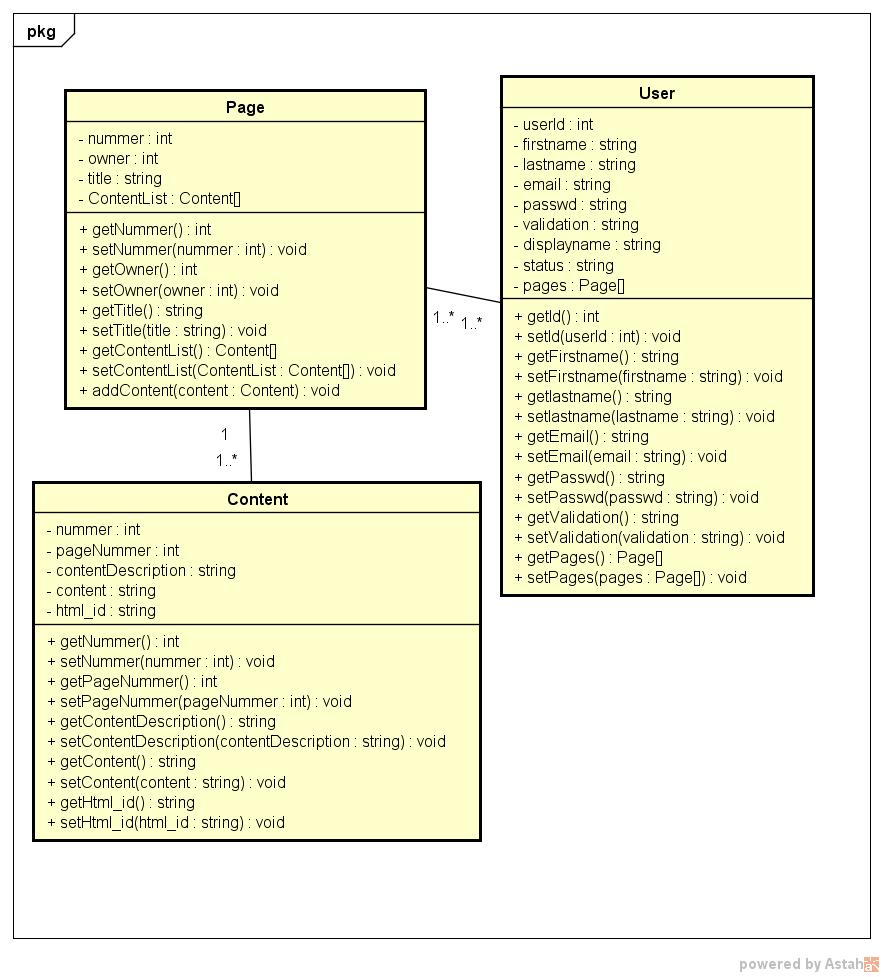
\includegraphics[width=\textwidth]{ClassDiagram}
\label{fig:classdiagram}
\end{figure}

\begin{figure}[h]
\caption{Datenmodell}
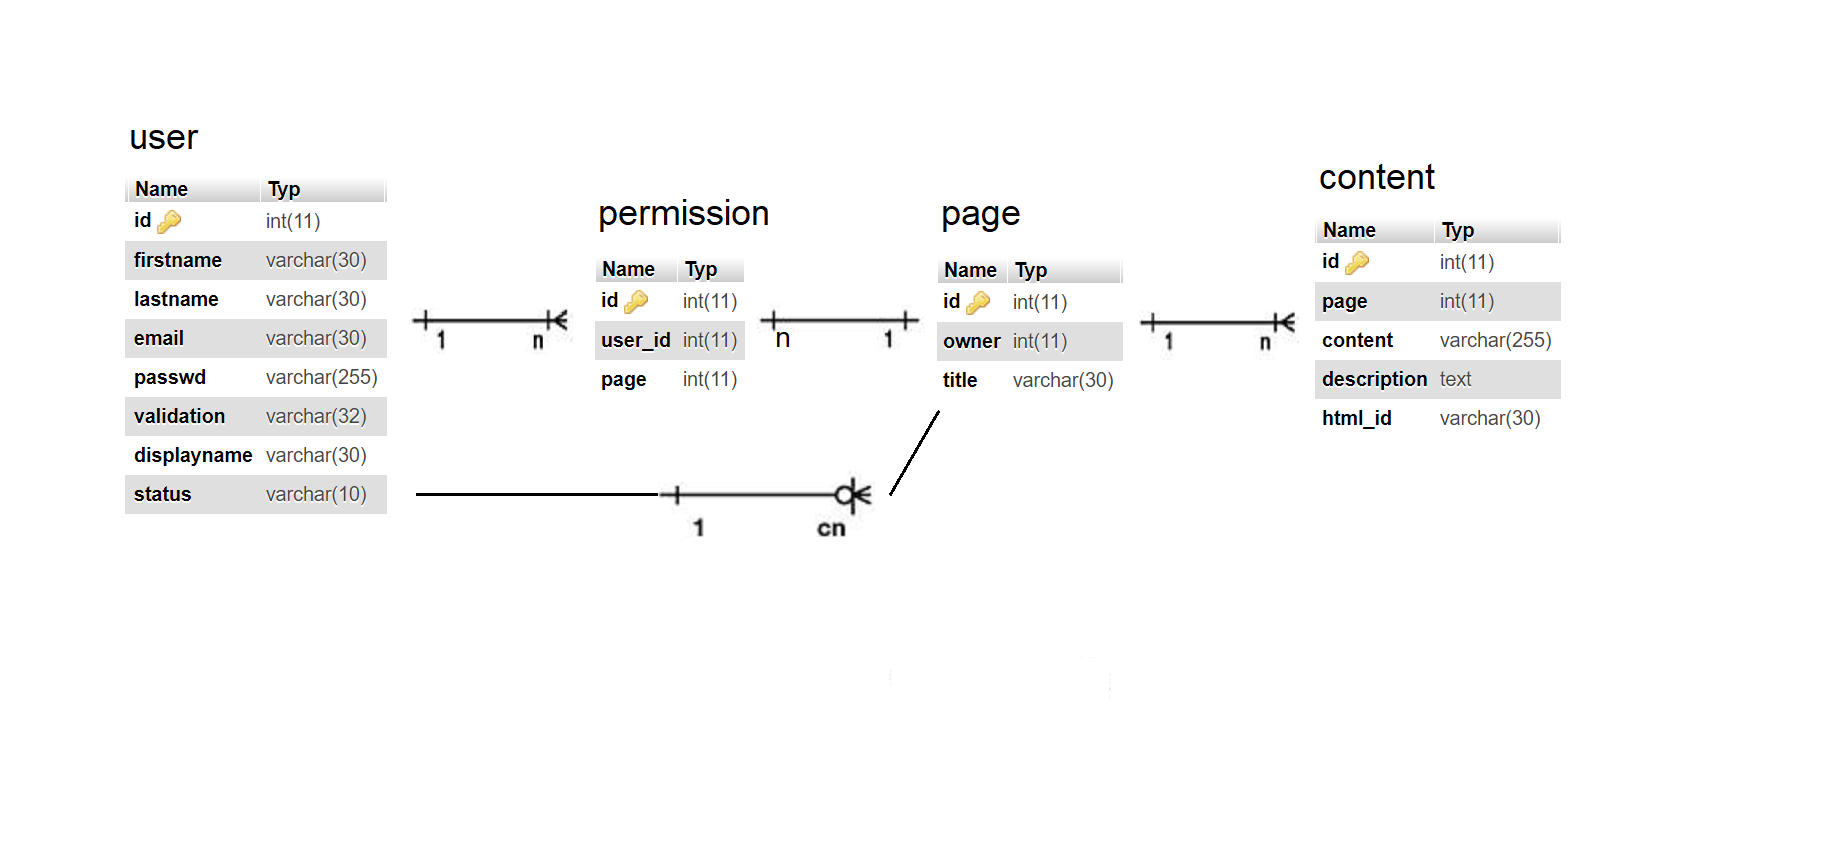
\includegraphics[width=\textwidth]{DatenmodellEPortfolio}
\label{fig:datenmodell}
\end{figure}

\begin{figure}[h]
\caption{Use Case Diagram}
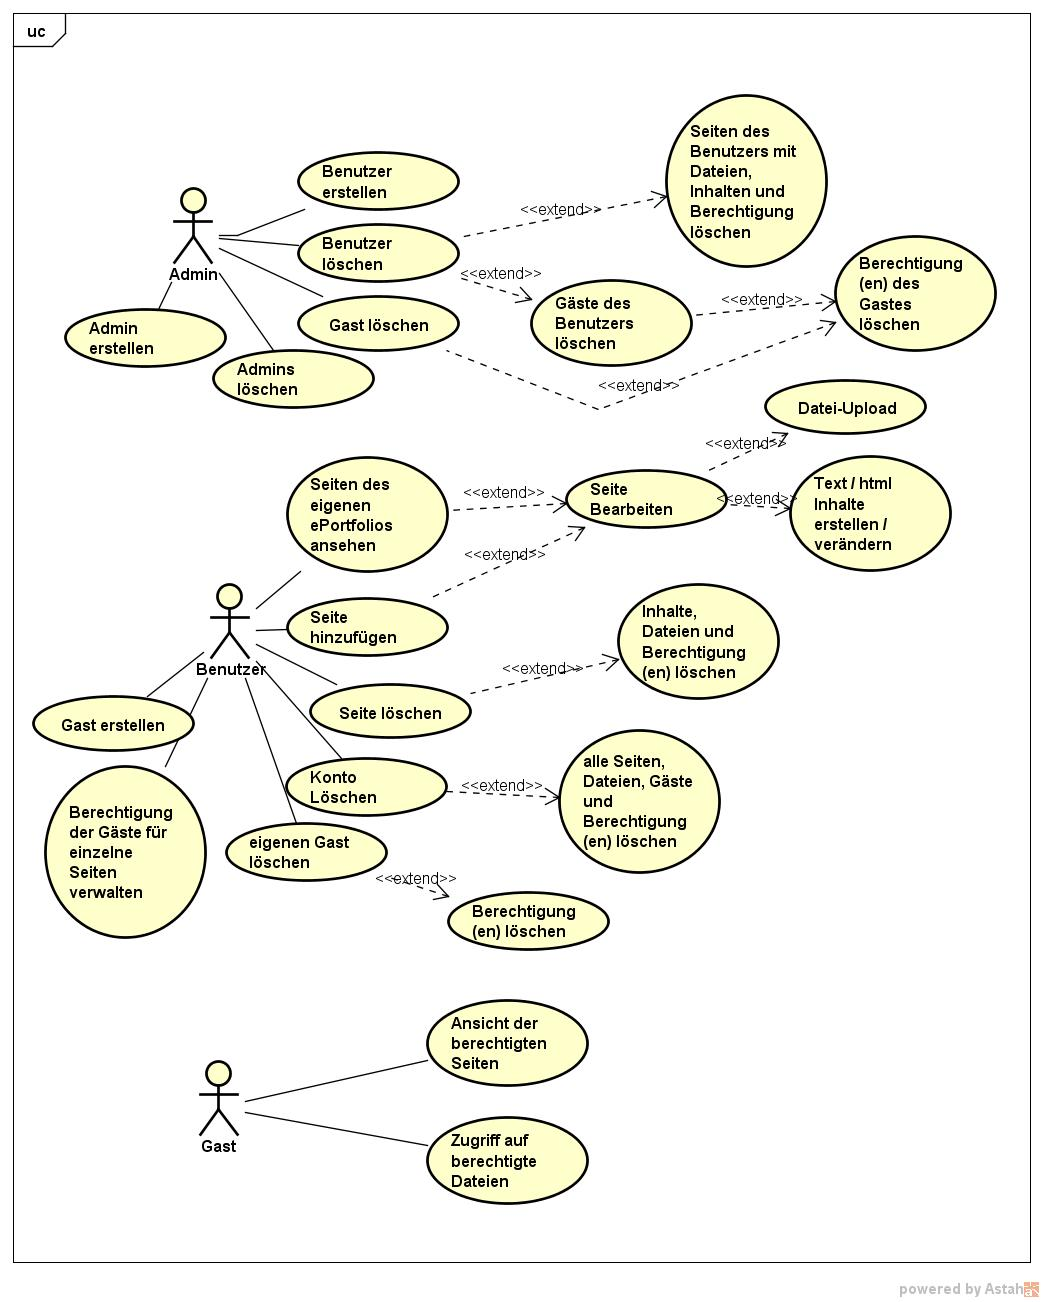
\includegraphics[width=\textwidth]{UseCaseDiagram}
\label{fig:usecasediagram}
\end{figure}



\end{document}